\documentclass[12pt, twoside]{article}
\usepackage[letterpaper, margin=1in, headsep=0.5in]{geometry}
\usepackage[english]{babel}
\usepackage[utf8]{inputenc}
\usepackage{amsmath}
\usepackage{amsfonts}
\usepackage{amssymb}
\usepackage{tikz}
\usetikzlibrary{quotes, angles}
\usepackage{graphicx}
\usepackage{enumitem}
\usepackage{multicol}

\newif\ifmeta
\metatrue %print standards and topics tags

\title{Regents Geometry}
\author{Chris Huson}
\date{September 2020}

\usepackage{fancyhdr}
\pagestyle{fancy}
\fancyhf{}
\renewcommand{\headrulewidth}{0pt} % disable the underline of the header
\raggedbottom


\fancyhead[LE]{\thepage}
\fancyhead[RO]{\thepage \\ Name: \hspace{4cm} \,\\}
\fancyhead[LO]{BECA / Dr. Huson / Geometry 01-Intro\\* pset ID: 7}

\begin{document}

\subsubsection*{1-4HW-Segment-addition}
\begin{enumerate}
\item I have a compass, ruler, protractor, notebook, and folder (circle one). Yes \qquad No

\item Use each term according to its geometric meaning: ``sketch", ``draw", ``construct".
    \begin{enumerate}
      \item $\rule{4cm}{0.15mm}$ is to make a freehand diagram showing important features. \smallskip
      \item $\rule{4cm}{0.15mm}$ is to depict with accurate measures using ruler, protractor, and compass. \smallskip
      \item $\rule{4cm}{0.15mm}$ is a formal, logical process to create geometric figures using only a straightedge and compass.
    \end{enumerate} \smallskip

\item Two or more line segments of equal measure are $\rule{4cm}{0.15mm}$.
    \bigskip
\item Given $\overline{ABC}$, $AB=10$, and $BC=4$.
  \begin{enumerate}
    \item Find ${AC}$.\\[0.75cm]
      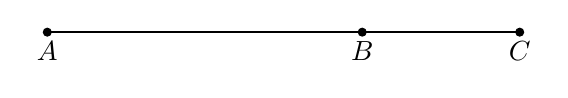
\begin{tikzpicture}
        \draw [-, thick] (1,0)--(7,0);
        \draw [fill] (1,0) circle [radius=0.05] node[below]{$A$};
        \draw [fill] (5,0) circle [radius=0.05] node[below]{$B$};
        \draw [fill] (7,0) circle [radius=0.05] node[below]{$C$};
      \end{tikzpicture} \smallskip
    \item The postulate used in this problem is the \rule{6cm}{0.15mm}.
  \end{enumerate}
  \smallskip

\item Given $\triangle ABC$ with $\overline{AC} \cong \overline{BC}$. On the diagram mark the congruent line segments with tick marks.
  \begin{center}
  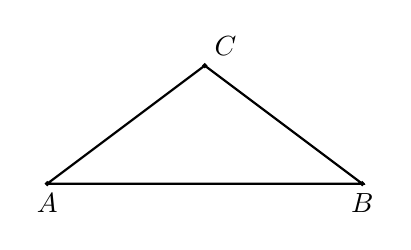
\begin{tikzpicture}[scale=0.5]
    \draw [thick](0,0)--(8,0)--(4,3)--(0,0);
    \draw [fill] (0,0) circle [radius=0.05] node[below]{$A$};
    \draw [fill] (8,0) circle [radius=0.05] node[below]{$B$};
    \draw [fill] (4,3) circle [radius=0.05] node[above right]{$C$};
  \end{tikzpicture}
  \end{center}

\item Given line segment $\overline{AB}$ with midpoint $M$, that is, $\overline{AM} \cong \overline{BM}$. $AM=2$ cm. Find the length of $\overline{AB}$.\\[0.75cm]
  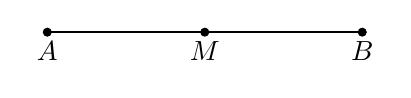
\begin{tikzpicture}
    \draw [-, thick] (1,0)--(5,0);
    \draw [fill] (1,0) circle [radius=0.05] node[below]{$A$};
    \draw [fill] (5,0) circle [radius=0.05] node[below]{$B$};
    \draw [fill] (3,0) circle [radius=0.05] node[below]{$M$};
  \end{tikzpicture}
  \vspace{1cm}

\item Points that are all located on the same line are $\rule{4cm}{0.15mm}$.

  \newpage
\item Given the points $X$ and $Y$, draw $\overrightarrow{YX}$.\\
  \vspace{1cm}
  \begin{center}
    \begin{tikzpicture}
    \draw [fill] (0,2) circle [radius=0.05] node[below]{$X$};
    \draw [fill] (5,0) circle [radius=0.05] node[below]{$Y$};
  \end{tikzpicture}
  \end{center}
  %\vspace{2cm}

\item Given $\triangle ABC$ write down two congruent line segments using proper notation.\\
  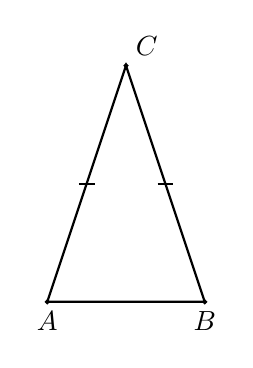
\begin{tikzpicture}[scale=0.5]
    \draw [thick](0,0)--(4,0)--(2,6)--(0,0);
    \draw [fill] (0,0) circle [radius=0.05] node[below]{$A$};
    \draw [fill] (4,0) circle [radius=0.05] node[below]{$B$};
    \draw [fill] (2,6) circle [radius=0.05] node[above right]{$C$};
    \draw [thick] (0.8,3)--(1.2,3); %tick mark
    \draw [thick] (2.8,3)--(3.2,3); %tick mark
  \end{tikzpicture}

\item Given $\overrightarrow{DE}$, construct circle $E$ with radius $DE$.
  \vspace{4cm}
  \begin{center}
  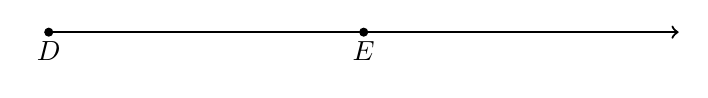
\begin{tikzpicture}
    \draw [->, thick] (0,0)--(8,0);
    \draw [fill] (0,0) circle [radius=0.05] node[below]{$D$};
    \draw [fill] (4,0) circle [radius=0.05] node[below]{$E$};
  \end{tikzpicture}
  \end{center}
  \vspace{4cm}
  Spicy: Complete the construction of an equilateral triangle with one side $\overline{DE}$.

\end{enumerate}
\end{document}